\documentclass[10pt,twocolumn,letterpaper]{article}

\usepackage{cvpr}
\usepackage{times}
\usepackage{epsfig}
\usepackage{graphicx}
\usepackage{amsmath}
\usepackage{amssymb}
\usepackage{array}
\usepackage{xfrac}
\usepackage{amssymb}
%\usepackage{todonotes}
\usepackage{centernot}
\usepackage{textcomp}
\usepackage{blindtext}
\usepackage{centernot}
\usepackage{wasysym}
\usepackage{siunitx}
\usepackage[letterpaper]{geometry}
\usepackage{color}
%\usepackage[table]{xcolor}
\usepackage{amsfonts}
\usepackage{mathtools}
\usepackage{multirow}
\usepackage[small,it]{caption}
%\usepackage{titling}
%\usepackage{filecontents}
%\usepackage{titlesec}
\usepackage[section]{placeins}
%\usepackage[hidelinks]{hyperref}
%\usepackage{fancyhdr}
\usepackage{cancel}
%\usepackage{abstract}
\usepackage{minted}
\usepackage{widetext}
\usepackage[utf8]{inputenc}

\sisetup{output-exponent-marker=\textsc{e}}

\DeclareMathOperator*{\argmax}{arg\,max}
\DeclareMathOperator*{\argmin}{arg\,min}

\newcommand{\squishlist}{
 \begin{list}{$\bullet$}
  { \setlength{\itemsep}{0pt}
     \setlength{\parsep}{3pt}
     \setlength{\topsep}{3pt}
     \setlength{\partopsep}{0pt}
     \setlength{\leftmargin}{1.5em}
     \setlength{\labelwidth}{1em}
     \setlength{\labelsep}{0.5em} } }


\newcommand{\squishlisttwo}{
 \begin{list}{$\bullet$}
  { \setlength{\itemsep}{0pt}
    \setlength{\parsep}{0pt}
    \setlength{\topsep}{0pt}
    \setlength{\partopsep}{0pt}
    \setlength{\leftmargin}{2em}
    \setlength{\labelwidth}{1.5em}
    \setlength{\labelsep}{0.5em} } }

\newcommand{\squishend}{
  \end{list}  }
\footskip = 50pt
\setlength{\skip\footins}{10pt}

\newcommand*{\vertbar}{\rule[-1ex]{0.5pt}{3.0ex}}
\newcommand*{\horzbar}{\rule[.5ex]{2.5ex}{0.5pt}}

% Include other packages here, before hyperref.

% If you comment hyperref and then uncomment it, you should delete
% egpaper.aux before re-running latex.  (Or just hit 'q' on the first latex
% run, let it finish, and you should be clear).
\usepackage[breaklinks=true,bookmarks=false]{hyperref}

\cvprfinalcopy % *** Uncomment this line for the final submission

\def\cvprPaperID{****} % *** Enter the CVPR Paper ID here
\def\httilde{\mbox{\tt\raisebox{-.5ex}{\symbol{126}}}}

% Pages are numbered in submission mode, and unnumbered in camera-ready
%\ifcvprfinal\pagestyle{empty}\fi
\setcounter{page}{1}
\begin{document}

%%%%%%%%% TITLE
\title{Pyramid Histograms of Visual Words}

\author{Edgar A. Margffoy-Tuay\\
Universidad de los Andes\\
201412566\\
{\tt\small ea.margffoy10@uniandes.edu.co}
% For a paper whose authors are all at the same institution,
% omit the following lines up until the closing ``}''.
% Additional authors and addresses can be added with ``\and'',
% just like the second author.
% To save space, use either the email address or home page, not both
%\and
%Second Author\\
%Institution2\\
%First line of institution2 address\\
%{\tt\small secondauthor@i2.org}
}

\maketitle
%\thispagestyle{empty}

%%%%%%%%% ABSTRACT
\begin{abstract}
Inspired by the Bag of Words representation used on Natural Language Processing, the Pyramid Histograms of Visual Words aims to represent an image as a set of local Visual Words, on which each visual word corresponds to a aggregation of SIFT features responses applied over several scales. This method allows to obtain remarkable results over uniform image classification benchmarks, such as Caltech-101, however it presents some flaws at the moment of applying it to more diverse datasets like ImageNet which reduces its accuracy.
\end{abstract}

%Segmentation represents one of the core Computer Vision tasks in scientfic and academic research since the 1970s, this problem is defined as the grouping of pixels on a image according to several semantic categories of interest. Until recently, this problem was approached by using pixel-level mathematical formulations based on classical image processing and DSP, without any association with other Computer Vision problems nor any AI-related task, such as NLP. However, after the rise of

%%%%%%%%% BODY TEXT
\section{Introduction}
%\subsection*{Context}
SIFT (Scale Invariant Feature Transform) descriptors were proposed by David Lowe \cite{Lowe:1999:ORL:850924.851523} on 1999 to describe local landmarks on images, these features are based on different operations, such as the calculation of Difference of Gaussian (DoG) at multiple scales and rotations and the Generalized Hough Transform, which result on descriptors of dimension 128 that are invariant to rotation and scaling, properties suitable to applications like 3D reconstruction and image projection. 
\\
\\
However, SIFT descriptors can be also used to represent an image on different scales and window areas, allowing to describe the input pixels as a combination of local SIFT responses, this allows to formulate higher level features that are more expressive than the pixel information alone. This process was exploited to achieve different results on other Computer Vision tasks different from those mentioned above, such as object recognition on which, SIFT-based methods like Pyramid Histograms of Visual Words achieved remarkable results on standard benchmarks such as Caltech-101, on which, this method achieved 70\% Accuracy \cite{Lazebnik:2006:BBF:1153171.1153549}.
\\
\\
This method is based on ideas used on Natural Language Processing, and more precisely, the Bag of Words representation. On which, each output vector is produced as a histogram of visual words, on which each visual word correspond to a centroid on the visual word dictionary conformed by clustering the Pyramid SIFT descriptors. Then, the histograms are classified using $N$ Support Vector Machines, one per each image class to discriminate. Overall, PHOW depends on several hyperparameters to accomplish the task such as the number of scales on which SIFT is going to be aggregated, other important parameter to consider is the number of visual words to cluster that depends on the parameter $K$ of K-Means, finally, the model depends on the regularization constant $C$ of the SVM classifiers.  
\\
\\
The election and setup of the model hyperparameters may affect the accuracy score over the dataser chosen. To address this variation issues, the present document aims to compare different image classification scores obtained after training a set of PHOW-based SVMs, subject to variations on their main hyperparameters.  Also, this report pretends to discuss the different results obtained after training a PHOW model subject to different parameters over the Caltech-101 and ImageNet datasets. 

\section{Materials and Methods}
To evaluate the accuracy of the PHOW approach to the Image Classification task, different sets of hyperparameters were evaluated over the Caltech-101\footnote{\url{http://www.vision.caltech.edu/Image_Datasets/Caltech101/}} \cite{fei2007learning} and a subset of 200 classes of ImageNet\footnote{\url{http://image-net.org/}} \cite{imagenet_cvpr09}. The parameters subject to adjustment were the spatial scale of the SIFT, the number of training and test cases to evaluate over the model, also, the number of visual words to cluster and finally, the regularization constant of the SVM was also subject to modifications. The parameters were chosen taking into account the computation limits of the processing machine which are subject to the size of the dataset to consider. For instance, to train the classifiers over ImageNet, a subset of 100 training images were used, due to the memory required to train the model using all the images. The PHOW implementation is based on VLFeat\footnote{\url{http://www.vlfeat.org/}} implementation done by Andrea Vedaldi \cite{vedaldi08vlfeat}.
\\
\\
Also, the parameter selection was based on the enviromental setting of each of the datasets chosen, for instance, Caltech-101 is based on uniform (Catalogue) images, which implies that the total required number of SIFT descriptor must be lower than the number of descriptors selected to train over ImageNet. All the datasets were evaluating using the mean of class comparison between the test ground truth labels and the model output labels. All the model configurations were evaluated over all the class labels included on both datasets.  
%\begin{figure*}[t]
%	\centering
%	%	\begin{center}
%	%\fbox{\rule{0pt}{2in} \rule{0.9\linewidth}{0pt}}
%	\epsfig{file=./Assets/Model_red.pdf,width=0.8\linewidth,clip=}
%	%\includegraphics[width=0.8\linewidth]{egfigure.eps}
%	%	\end{center}
%	\caption{Visual description of the planned baseline to approach the image segmentation recovery problem given a video input. Images taken by the author}
%	\label{Fig:F1}
%	%\label{fig:long}
%	%\label{fig:onecol}
%\end{figure*}


\section{Results}
\begin{table*}
	\centering
	\begin{tabular}{|c|c|c|c|c|c|c|}
		\hline
		\multicolumn{7}{|c|}{Caltech-101} \\
		\hline
		\# Train & \# Test & \# Words & Spatial-X & Spatial-Y & $C$ & Accuracy (\%) \\
		\hline
		20 & 20 & 600 & (2, 4) & (2, 4) & 10 & 70.85\% \\
		\hline
		50 & 20 & 1000 & (2, 4) & (2, 4) & 10 & \textbf{75.79}\% \\
		\hline
		50 & 20 & 600 & (2, 4) & (2, 4) & 30 & 75.37\% \\
		\hline
		50 & 20 & 600 & (2, 4) & (2, 4) & 5 & 74.94\% \\
		\hline
	\end{tabular}
	\caption{Caltech-101: Accuracy test results of PHOW subject to different hyperparameter configurations}
	\label{Tab:Cal}
\end{table*}

\begin{table*}
	\centering
	\begin{tabular}{|c|c|c|c|c|c|c|}
		\hline
		\multicolumn{7}{|c|}{ImageNet-200} \\
		\hline
		\# Train & \# Test & \# Words & Spatial-X & Spatial-Y & $C$ & Accuracy (\%) \\
		\hline
		50 & 100 & 1000 & (2, 5) & (2, 5) & 10 & 24.47\% \\
		\hline
		50 & 100 & 600 & (2, 4) & (2, 4) & 10 & 23.24\% \\
		\hline
		70 & 100 & 1200 & (1, 5) & (1, 5) & 10 & \textbf{27.17}\% \\
		\hline
	\end{tabular}
	\caption{ImageNet-200: Accuracy test results of PHOW subject to different hyperparameter configurations}
	\label{Tab:ImageNet}
\end{table*}

After evaluating the model over the proposed datasets, it is possible to appreciate in first place that the accuracy test scores associated to the PHOW evaluation over Caltech-101 were greater (Table~\ref{Tab:Cal}) than the scores obtained after evaluating similar PHOW parameter sets over the test set of ImageNet-200 (Table~\ref{Tab:ImageNet}), this is due to the increase in the number of classes and the difference between the main characteristics of the images present on both data sets, while in the former all images have regular lightning, scales and uniform backgrounds, the latter dataset considers all possible anomalies of interest at the moment of tackling an image classification problem. The main differences between the datasets presented previously consist of visual occlusion, scale deformations and intra-class differences, with respect to the latter condition, it is possible to appreciate that ImageNet exploits the hierarchic organization of the images according to upper (Less especific) and lower (More especific) categories, which allows to discriminate especific intra-class appereance, whereas on Caltech-101 each image set class is restricted to a single umbrella category.
\\
\\
This difference allows to exploit the inner properties of SIFT on a uniform set of images like Caltech-101, on which it is expected that all dogs share the same keypoints on all images, whereas on ImageNet this representation is ambiguous due to the presence of intra-class image appereances. For instance, the PHOW descriptors may be similar for both German Shepherd and American Staffordshire Terrier, which cannot give insights or more information about how to distinguish both dog breeds especifically, which implies an increase on the total number of False Positives present per class.
\\
\\
With respect to the hyperparameter selection and definition, it is possible to conclude that the model accuracy is influenced mainly by three parameters, namely, the number of training images used to conform the Visual Words Dictionary, also the total number of visual words to cluster and finally, the spatial configuration of each SIFT Pyramid to calculate.  As it can be deduced from Table~\ref{Tab:Cal}, an increase on the total number of visual words to consider, reflects an increase on the total class prediction accuracy percentage, however this number is subject to the main downsides of K-Means initialization, such as the convexity of each cluster and total number of dense SIFT descriptors, \textit{i.e.,} The more visual words are defined, the probabiility of obtaining empty or single descriptor words increases.
\\
\\
The total number of training images influence the accuracy model because they allow to grab and compile more input features that may contribute to the total distribution of visual words and the classification process as well, however, an increase on the number of training images must be done taking in account other parameters, such as the spatial distribution of the pyramids (\textit{i.e.,} Size), which allow to capture more scale feature information, which in turn can be used to discriminate better similar classes, however, this process is done at the expense of more memory consumption.
\\
\\
Finally, after evaluating the best model configurations as presented on the Tables~\ref{Tab:Cal} and \ref{Tab:ImageNet}, it was possible to appreciate that the Waterlilly (Caltech-101) and African Elephant (ImageNet) were among the most difficult object categories to recognize, due to their color, scale and appereance ambiguity that allows them to be recognized as other objects and not precisely as the original one. Other categories such as barrel are easy to recognize, due to the presence of a definite shape, scale ratio and color.

\section{Conclusions}
The PHOW model is a very expressive tool, suitable to classification of uniform images and definite classes without any visual occlussion nor any scale anomality, due to SIFT's properties, which allow to describe images as a set of features that are Scale and Rotation invariant. However, the objects must be positioned and visible inside the image to satisfy those conditions.
\\
\\
As it was concluded after evaluating this model over non uniform datasets like ImageNet, PHOW formulation is weak at the moment of classifying different class instances of the same global class (Like dog breeds), because dense SIFT descriptors tend to be similar between those classes, which in turn introduces ambiguity to the classifier, and eventually, the dominance of a class over others. This behaviour was observed over all the experiments formulated, independent of the set of hyperparameters chosen, that allows us to conclude that as one of the main limitations of the PHOW approach to image classification.
\\
\\
The improvement of the model may be based on a modification of the visual word coding process, which can be abstracted from K-Means, this new formulation should aim to remove the side effects introduced by employing other visual dictionary conformation techniques, that allow to replace the K-Means introduction. Also, it is possible to refine the vector representation of each dense SIFT by adding more information, like dense SIFT applied to all color channels. It is also possible to combine SIFT descriptors with other feature representations, such as Speeded Up Robust Features (SURF) \cite{bay2006surf}. Finally, the classifier can be replaced in order to use more robust models, such as Neural Networks, Deep Belief Networks and Random Forests. 


{\small
\bibliographystyle{ieee}
\bibliography{egbib}
}


\newpage
%\section{Some Results}
%\begin{figure}[H]
%	\centering
%	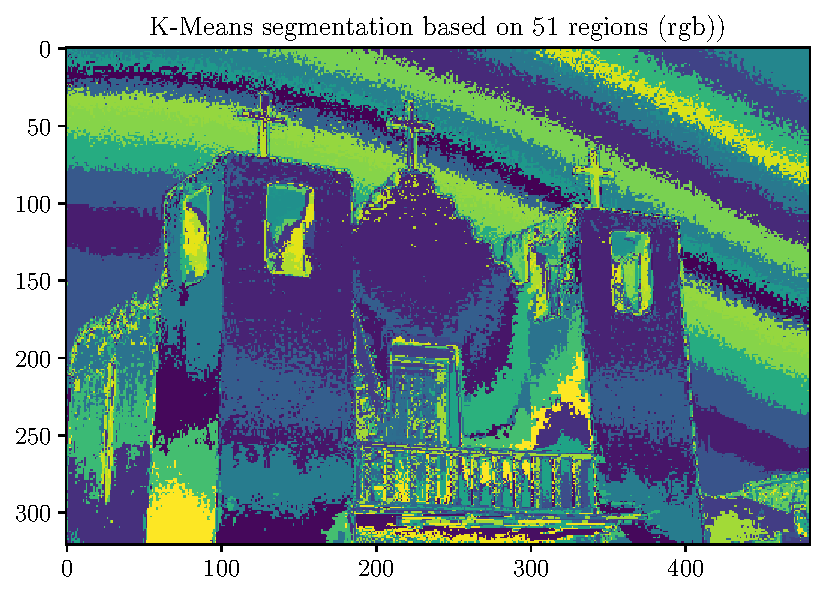
\epsfig{file=./Assets/24063_k-means_rgb_51.pdf,width=1.0\linewidth,clip=}
%	\caption{Example of K-Means segmentation result subject to 51 regions (No spatial)}
%	\label{Fig:kmeans1}
%\end{figure}
%
%
%\begin{figure}[H]
%	\centering
%	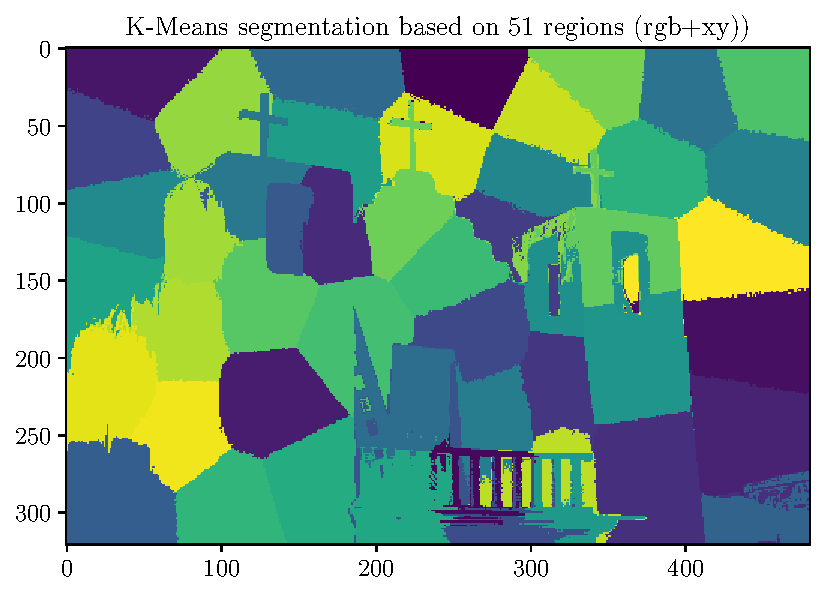
\epsfig{file=./Assets/24063_k-means_rgb+xy_51.pdf,width=1.0\linewidth,clip=}
%	\caption{Example of K-Means segmentation result subject to 51 regions (Spatial), this figure presents a large number of convex and spherical regions}
%	\label{Fig:kmeans2}
%\end{figure}
%
%\begin{figure}[H]
%	\centering
%	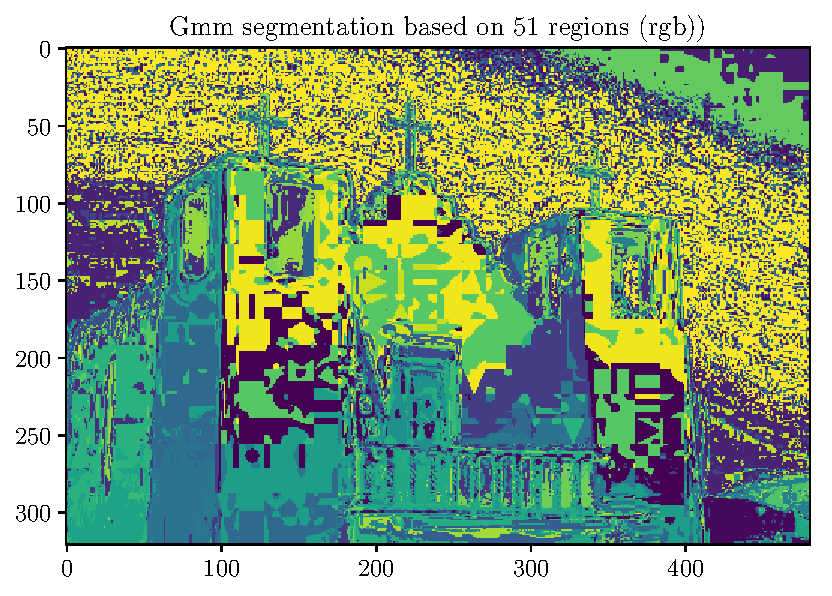
\epsfig{file=./Assets/24063_gmm_rgb_51.pdf,width=1.0\linewidth,clip=}
%	\caption{Example of GMM segmentation result subject to 51 regions (No spatial)}
%	\label{Fig:gmm1}
%\end{figure}
%
%\begin{figure}[H]
%	\centering
%	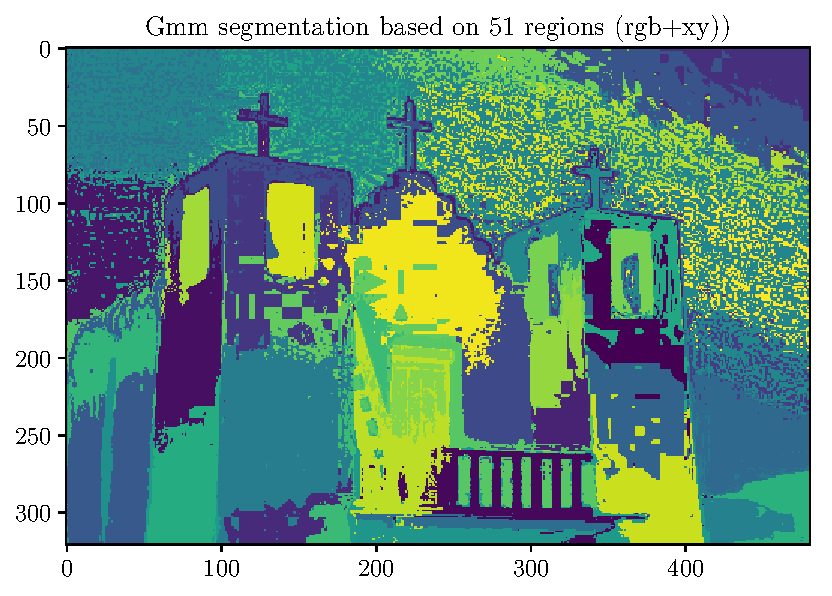
\epsfig{file=./Assets/24063_gmm_rgb+xy_51.pdf,width=1.0\linewidth,clip=}
%	\caption{Example of GMM segmentation result subject to 51 regions (Spatial information added), the noise was reduced}
%	\label{Fig:gmm2}
%\end{figure}
%
%\begin{figure}[H]
%	\centering
%	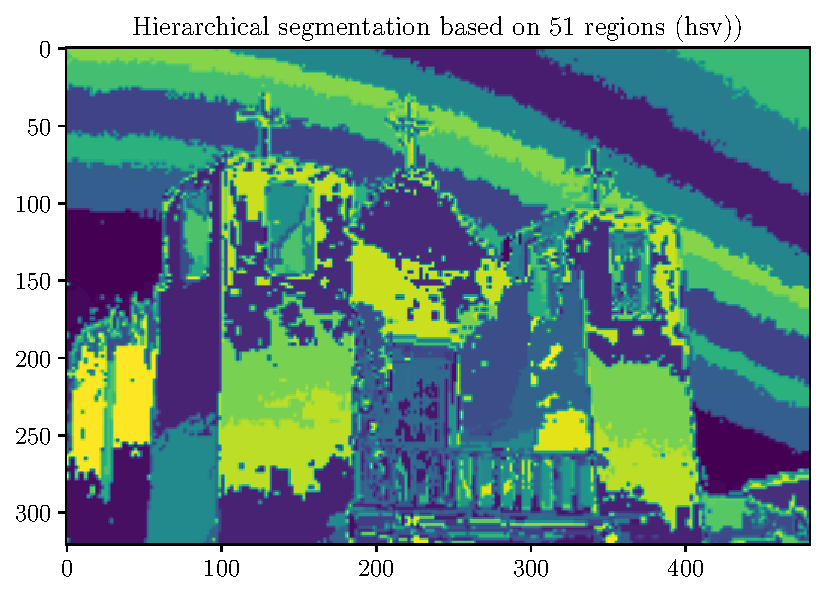
\epsfig{file=./Assets/24063_hierarchical_hsv_51.pdf,width=1.0\linewidth,clip=}
%	\caption{Example of Hierarchic segmentation result subject to 51 regions (No spatial information added), notice the smooth noise throughout all the regions by interpolation effects}
%	\label{Fig:hier1}
%\end{figure}
%
%\begin{figure}[H]
%	\centering
%	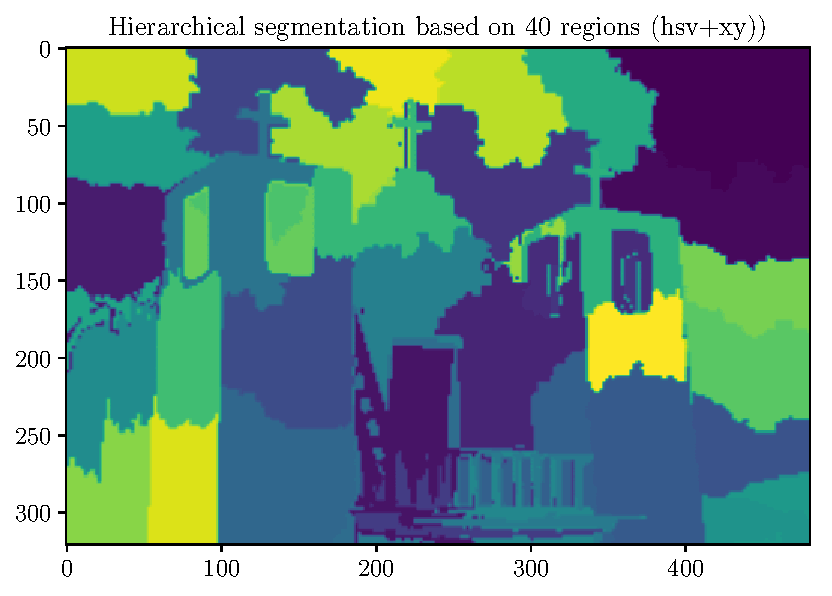
\epsfig{file=./Assets/24063_hierarchical_hsv+xy_40.pdf,width=1.0\linewidth,clip=}
%	\caption{Example of Hierarchic segmentation result subject to 40 regions (Spatial information added), notice the smooth noise throughout all the regions by interpolation effects}
%	\label{Fig:hier2}
%\end{figure}
%
%\begin{figure}[H]
%	\centering
%	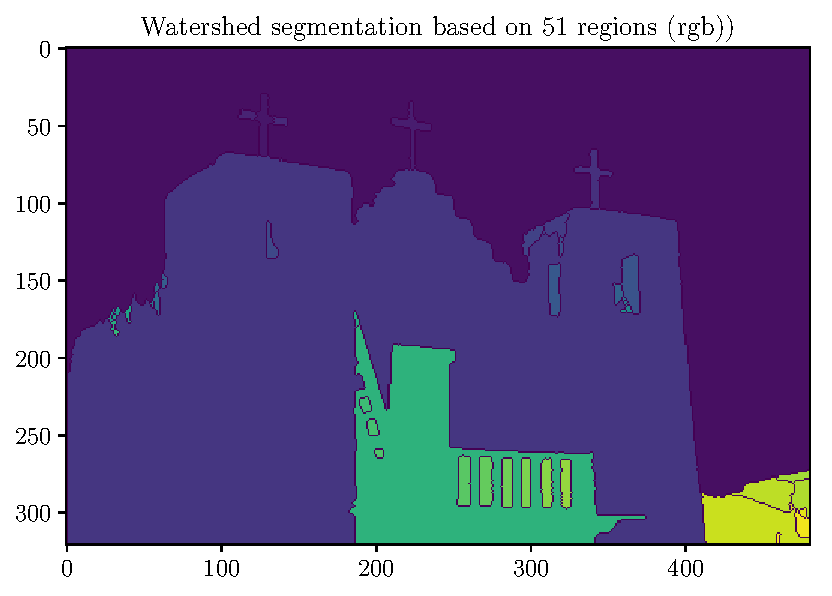
\epsfig{file=./Assets/24063_watershed_rgb_51.pdf,width=1.0\linewidth,clip=}
%	\caption{Example of H-Minima Watershed segmentation result subject to 51 regions, notice the well defined contours and regions}
%	\label{Fig:water1}
%\end{figure}
%
%\begin{figure}[H]
%	\centering
%	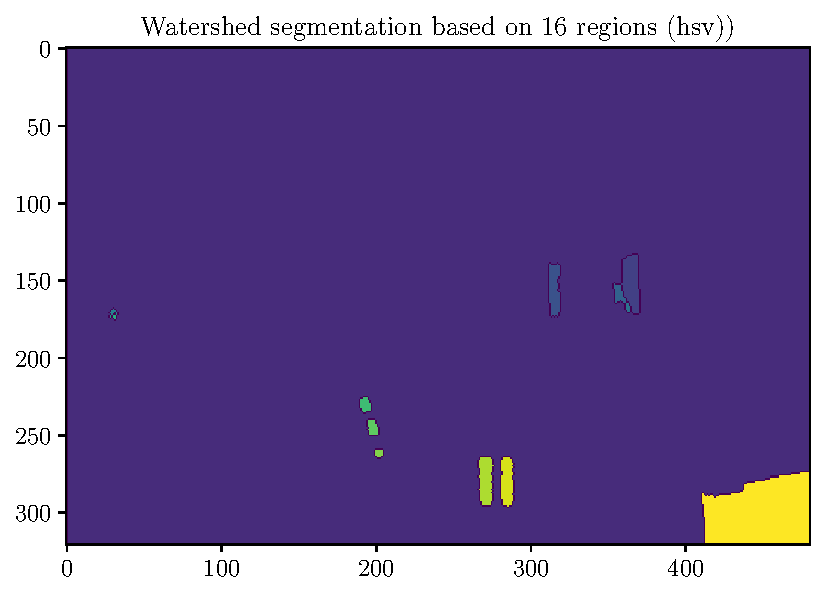
\epsfig{file=./Assets/24063_watershed_hsv_16.pdf,width=1.0\linewidth,clip=}
%	\caption{Example of H-Minima Watershed segmentation result subject to 16 regions, notice the disappearance of the main ROI}
%	\label{Fig:water2}
%\end{figure}



\end{document}
